\documentclass[portrait,final,a0paper,fontscale=0.3]{baposter}

\usepackage[utf8]{inputenc}
\usepackage[T1]{fontenc}
\usepackage[frenchb]{babel} 

\usepackage{graphicx}
\usepackage{multirow}
\usepackage{enumitem}
\usepackage{url}

\usepackage{graphicx}
\usepackage{multicol}

\usepackage{palatino}

\usepackage{wasysym}

\newcommand{\captionfont}{\footnotesize}

\frenchbsetup{ItemLabeli=\textbullet}
\frenchbsetup{ItemLabelii=\normalfont \bfseries \textendash}
\frenchbsetup{ItemLabeliii=\textasteriskcentered}
\frenchbsetup{ItemLabeliv=\textperiodcentered}

% Multicol Settings
%%%%%%%%%%%%%%%%%%%%%%%%%%%%%%%%%%%%%%%%%%%%%%%%%%%%%%%%%%%%%%%%%%%%%%%%%%%%%%%%
\setlength{\columnsep}{1.5em}
\setlength{\columnseprule}{0mm}

%%%%%%%%%%%%%%%%%%%%%%%%%%%%%%%%%%%%%%%%%%%%%%%%%%%%%%%%%%%%%%%%%%%%%%%%%%%%%%%%
\newcommand{\compresslist}{%
\setlength{\itemsep}{1pt}%
\setlength{\parskip}{0pt}%
\setlength{\parsep}{0pt}%
}
\setlist{leftmargin=5.5mm}

\definecolor{darkblue}{rgb}{0.1,0.2,0.5}
\definecolor{darkred}{rgb}{0.7,0,0.0}
\definecolor{darkgreen}{rgb}{0.0,0.4,0.0}
\definecolor{darkmagenta}{rgb}{0.4,0.0,0.4}
\definecolor{darkcyan}{rgb}{0.0,0.5,0.5}
\definecolor{darkyellow}{rgb}{1,0.5,0.0}
\definecolor{darkgray}{rgb}{0.2,0.2,0.2}
\definecolor{lightgray}{rgb}{0.9,0.9,0.9}
\definecolor{verylightgray}{rgb}{0.95,0.95,0.95}
\definecolor{ensggreen}{rgb}{0.50,0.63,0.05}
\definecolor{ensggray}{rgb}{0.45,0.47,0.49}
\definecolor{lightgreen}{rgb}{0.0,0.9,0.0}
\definecolor{lightred}{rgb}{0.9,0.0,0.0}
\definecolor{lightblue}{rgb}{0.0,0.0,0.9}


\renewenvironment{emph}[1]{\textbf{#1}}{}
\graphicspath{{../Rapport/imgs/}}

\begin{document}

\hyphenation{resolution occlusions}
\begin{poster}%
	% Poster Options
	{
	columns=6,
	% Column spacing
	colspacing=0.7em,
	% Color style
	bgColorOne=white,
	borderColor=darkblue,
	headerColorOne=darkblue,
	headerFontColor=white,
	boxColorOne=white,
	% Format of textbox
	textborder=roundedsmall,
	% Format of text header
	headerborder=closed,
	headerheight=0.1\textheight,
	%  textfont=\sc, An example of changing the text font
	headershape=smallrounded,
	headershade=plain, %shadelr,
	headerfont=\Large\bf\textsc, %Sans Serif
	textfont={\setlength{\parindent}{1.5em}},
	boxshade=plain,
	background=plain, %shadetb
	linewidth=2pt
	}
	% Logo1
	% {
\includegraphics[height=9.0em]{ensta_bzh.png}}
	{
\includegraphics[height=3.0em]{logo_ensta.jpg}
	
\includegraphics[height=3.0em]{logo-lab-sticc2.png}
	
\includegraphics[height=3.0em]{logo_ubs_transparent.png}}
	% Title
	{\bf\textsc{Docking autonome pour un USV}\vspace{0.5em}}
	% Authors
	{\normalsize\textsc{\textbf{\underline{GROUPE :}} Hugo HOFMANN$^{(1)}$, Guillaume GARDE$^{(1)}$, Kevin REN$^{(1)}$, Théo MASSA$^{(1)}$}\vspace{0.5em}
	\\\normalsize\textsc{\textbf{\underline{ENCADRANTS :}} Ronan DOUGUET$^{(1)}$, Yvan EUSTACHE$^{(1)}$, Dominque HELLER$^{(1)}$}\vspace{0.5em}
	\\$(1)$ ENSTA Bretagne ; $(2)$ UBS
	\vspace{-0.25cm}}
	% Logo2
	{}

%%%%%%%%%%%%%%%%%%%%%%%%%%%%%%%%%%%%%%%%%%%%%%%%%%%%%%%%%%%%%%%%%%%%%%%%%%%%%%
\headerbox{Contexte}{name=contexte,column=0,span=4}{
%%%%%%%%%%%%%%%%%%%%%%%%%%%%%%%%%%%%%%%%%%%%%%%%%%%%%%%%%%%%%%%%%%%%%%%%%%%%%%
	\setlength{\parindent}{0pt}
	Que ce soit dans le monde de la recherche ou dans les différents domaines dans lesquels
	sont utilisés les drones et tout particulièrement les AUV ou UAV, l’une des grandes difficultés
	rencontrées est très certainement celle du docking. En effet, cela peut se révéler dans le meilleur des
	cas fastidieux (dans le cas ou la manoeuvre est manuelle par exemple) et dans le pire des cas
	difficile voire dangereux pour le drone (dans le cas d’une mer agitée par exemple). Dans le
	cas d’une mission autonome loin du bateau, on comprend qu’il peut être très intéressant de
	développer une solution de docking autonome, permettant au drone de revenir vers sa base tout
	seul et avec précision. L’objectif de ce projet Guerlédan sera donc de développer cette solution
	en s’intéressant au cas d’un AUV sur le lac.
}

\headerbox{Objectifs}{name=resume,column=4,span=2}{
	\setlength{\parindent}{0pt}
	
	\vspace{2mm}
	\begin{center}
		\textcolor{red}{\emph{Concevoir une architecture permettant
		\\un docking autonome}}
	\end{center}
	
	\vspace{-1mm}
	Points essentiels :
	\begin{itemize}
		\item Planifier et réaliser le retour vers le dock.
		\item Assurer la communication drone-dock.
		\item Assurer une précision suffisante.
	\end{itemize}
}

\headerbox{Matériel}{name=methodologie,column=0,below=contexte,span=6}{
	\setlength{\parindent}{0pt}
	\centering Le projet se décompose en 3 parties essentielles
	
	\begin{minipage}[t]{0.30\textwidth}
		\vspace{-0.1cm}
		\begin{center}
			\large\textcolor{red}{\emph{Drone}}
		\end{center}
		\small\vspace{-0.2cm}
		L'USV est le \textit{M1800 d'IMSolutions}. Il contient toute une batterie de capteur,
		mais nous utiliserons seulement sa centrale inertielle \textit{SBG Ellipse D}, ainsi
		que le GPS à double antenne.
		\begin{center}
			\includegraphics*[width=0.75\textwidth]{monodrone-1800-chenal.jpg}
		\end{center}
	\end{minipage}\hfill
	\begin{minipage}[t]{0.30\textwidth}
		\vspace{-0.1cm}
		\begin{center}
			\large\textcolor{green}{\emph{Dock}}
		\end{center}
		\small\vspace{-0.2cm}
		L'électronique du dock est concentré dans une boite étanche. Elle est composée d'une \textit{NVIDIA
		Jetson Nano}, une centrale inertielle \textit{SBG Ellipse A}, un récepteur GNSS \textit{ublox} monté
		sur une carte \textit{ArduSimple},un modem \textit{SIMPULSE} pour la communication avec le drone
		et une antenne radio \textit{Xbee} pour recevoir les corrections RTK.
		\begin{center}
			\includegraphics*[height=0.8\textwidth,angle=90]{dock_box_outside.jpg}
		\end{center}
	\end{minipage}\hfill
	\begin{minipage}[t]{0.30\textwidth}
		\vspace{-0.1cm}
		\begin{center}
			\large\textcolor{blue}{\emph{Rover}}
		\end{center}
		\small\vspace{-0.2cm}
		Un rover \textit{AION R1} de \textit{AION Robotics}, fourni pour tester nos algorithmes à l'école,
		où nous n'avions pas accès au drone.
		\begin{center}
			\includegraphics*[width=0.55\textwidth]{rover.jpg}
		\end{center}
	\end{minipage}
}

\headerbox{Stratégie d'approche}{name=initialisation,column=0,below=methodologie,span=3}{
	\setlength{\parindent}{0pt}

	% Bloc 1
	\begin{center}
		\textbf{Filtre de Kalman}
	\end{center}
	\vspace{-0.3cm}
	Afin d'améliorer notre approche et compenser les différentes fréquences capteurs ainsi qu'incertitudes,
	nous avons décidé d'implémenter un filtre de Kalman en partant du modèle cinématique suivant:
	\begin{eqnarray*}
		\label{eq:cinematic} \left( \begin{array}{c}
		  \dot{x}\\
		  \dot{y}\\
		  \dot{z}\\
		  \dot{\psi}
		\end{array} \right) & = & \left( \begin{array}{cc}
		  \cos (\varphi) \cos (\psi) & 0\\
		  \cos (\varphi) \sin (\psi) & 0\\
		  - \sin (\varphi) & 0\\
		  0 & 1
		\end{array} \right) \left( \begin{array}{c}
		  v\\
		  \omega
		\end{array} \right) 
	\end{eqnarray*}

	Avec $(x,y,z)$ la position du drone dans le repère ENU, $\varphi$ l'assiette et $\psi$ le cap. Ici,
	le modèle est issu de celui de Dubins, contrôlé en vitesse linéaire et angulaire sur le cap, étant
	donné que le contrôle du drone se fait de cette manière.
	
	\begin{minipage}[t]{0.49\textwidth}
		\vspace{-0.1cm}
		\begin{center}
			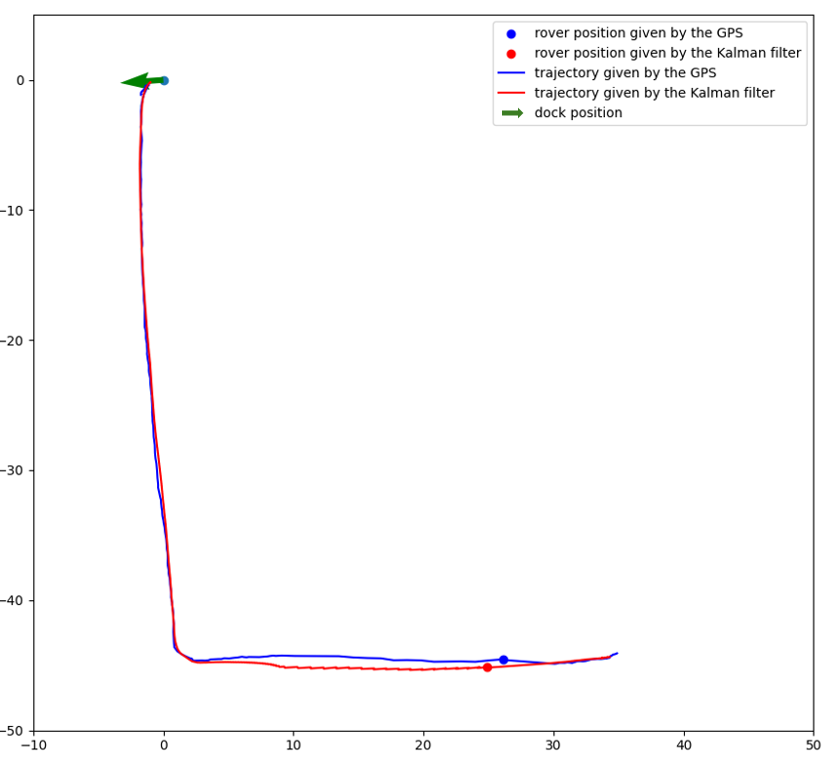
\includegraphics[width=0.9\textwidth]{GPSvsKalman.png}
		\end{center}
	\end{minipage}\hfill
	\begin{minipage}[t]{0.49\textwidth}
		\vspace{-0.1cm}
		Ici, on peut comparer la position brute renvoyée par le GPS et
		la position estimée renvoyée par notre filtre de Kalman. Cette comparaison
		correspond à un docking attenté avec le rover sur le stade de l'ENSTA.\linebreak
		Les deux positions restent proches, mais l'utilisation de Kalman, notamment la partie
		prédictive du filtre, permet de compenser la faible fréquence de mise à jour des
		données GPS.
	\end{minipage}\hfill


    % Séparation verticale
    \vspace{\baselineskip}
	
    % Bloc 2
	\begin{center}
		\textbf{Guidage par champ de potentiel}
	\end{center}
	\vspace{-0.3cm}

	L'approche se fait en deux phases selon la position initiale. Si il se situe derrière le dock,
	le drone va vouloir se placer du bon côté puis entamer sa procédure de docking. Dans le premier cas,
	le champ est constant dans la direction du cap du dock, dans le second, on considère une ligne attractive
	alignée sur le dock.

	\begin{center}
		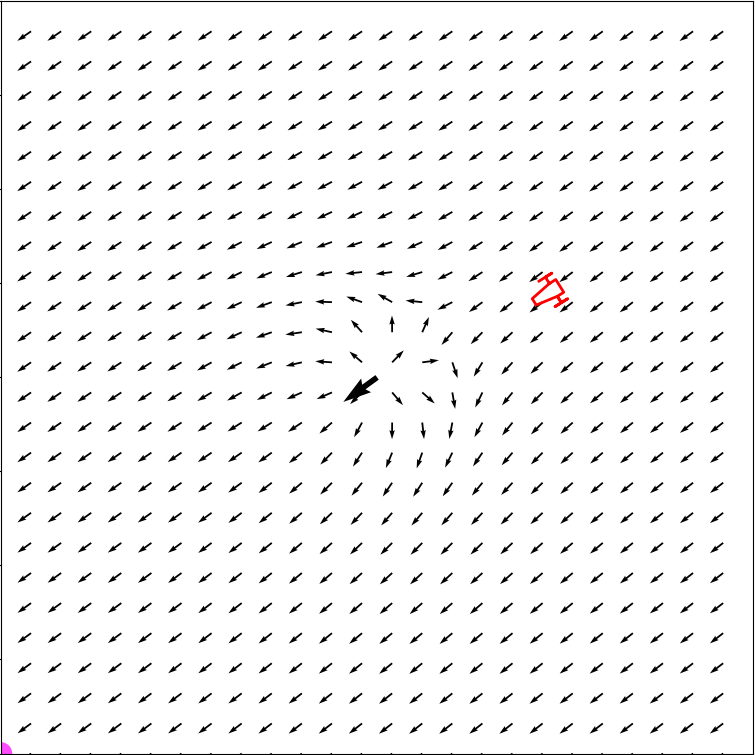
\includegraphics[width=0.25\textwidth]{ScreenshotCase2.png}
		\hfil
		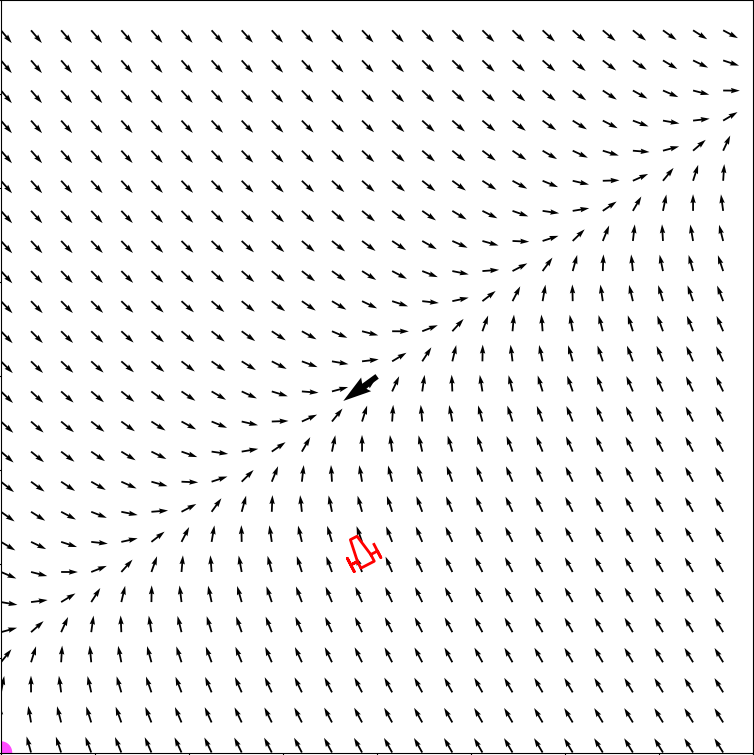
\includegraphics[width=0.25\textwidth]{ScreenshotCase1.png}
		
		A gauche, la phase de mise en place, à droite, la phase de docking
	\end{center}
}

\headerbox{architecture logicielle}{name=dynamique,column=3,below=methodologie,span=3}{
	\setlength{\parindent}{0pt}\small\smallskip

	Pour ce projet, nous avons travaillé sous \textit{ROS Melodic}. Du aux contraintes inhérentes
	au middleware, nous avons estimé qu'il était plus simple que le dock et le drone communiquent
	via des trames UDP.

	\begin{center}
		\includegraphics*[width=0.7\textwidth]{schema_general.png}
	\end{center}	
}

\headerbox{Conclusion}{name=conclusion,column=3,below=dynamique, span=3}{
	Ci-dessous l'algorithme essayé sur le stade de l'ENSTA avec le rover.
	\begin{center}
		\includegraphics*[width=0.5\textwidth]{visu_1.png}
	\end{center}

	\vspace{-0.1cm}
	Cependant, il peut être intéressant pour la suite d'améliorer le processus en utilisant d'autres
	capteurs qu'uniquement la centrale inertielle et le GPS. On pourrait par exemple utiliser une caméra et un
	capteur lidar une fois assez proche du dock pour plus de précision.

}

\headerbox{}{name=conclusion,column=3,below=conclusion, span=3}{
	\setlength{\parindent}{0pt}\small\smallskip
	Les auteurs tiennent à remercier :
	\begin{itemize}
		\item La base nautique de Guerlédan pour leur accueil.
		\item Nos encadrants pour leur aide et disponibilité au cours du projet.
		\item Simon Rohou pour l'organisation de tout le projet Guerlédan.
	\end{itemize}
	
	\vspace{0.03cm}
	Cette étude a été réalisée durant l'année scolaire 2023-2024 dans le cadre du projet Guerlédan de 3ème année du cycle Ingénieur de l'ENSTA Bretagne, spécialité "Robotique".
}

\end{poster}
\end{document}